%% abtex2-modelo-trabalho-academico.tex, v-1.9.2 laurocesar
%% Copyright 2012-2014 by abnTeX2 group at http://abntex2.googlecode.com/ 
%%
%% This work may be distributed and/or modified under the
%% conditions of the LaTeX Project Public License, either version 1.3
%% of this license or (at your option) any later version.
%% The latest version of this license is in
%%   http://www.latex-project.org/lppl.txt
%% and version 1.3 or later is part of all distributions of LaTeX
%% version 2005/12/01 or later.
%%
%% This work has the LPPL maintenance status `maintained'.
%% 
%% The Current Maintainer of this work is the abnTeX2 team, led
%% by Lauro César Araujo. Further information are available on 
%% http://abntex2.googlecode.com/
%%
%% This work consists of the files abntex2-modelo-trabalho-academico.tex,
%% abntex2-modelo-include-comandos and abntex2-modelo-references.bib
%%

% ------------------------------------------------------------------------
% ------------------------------------------------------------------------
% abnTeX2: Modelo de Trabalho Academico (tese de doutorado, dissertacao de
% mestrado e trabalhos monograficos em geral) em conformidade com 
% ABNT NBR 14724:2011: Informacao e documentacao - Trabalhos academicos -
% Apresentacao
% ------------------------------------------------------------------------
% ------------------------------------------------------------------------

\documentclass[
	% -- opções da classe memoir --
	12pt,				% tamanho da fonte
	openright,			% capítulos começam em pág ímpar (insere página vazia caso preciso)
	oneside,			% para impressão em verso e anverso. Oposto a oneside
	a4paper,			% tamanho do papel. 
	% -- opções da classe abntex2 --
	%chapter=TITLE,		% títulos de capítulos convertidos em letras maiúsculas
	%section=TITLE,		% títulos de seções convertidos em letras maiúsculas
	%subsection=TITLE,	% títulos de subseções convertidos em letras maiúsculas
	%subsubsection=TITLE,% títulos de subsubseções convertidos em letras maiúsculas
	% -- opções do pacote babel --
	english,			% idioma adicional para hifenização
	french,				% idioma adicional para hifenização
	spanish,			% idioma adicional para hifenização
	brazil				% o último idioma é o principal do documento
	]{abntex2}

% ---
% Pacotes básicos 
% ---
%\usepackage{lmodern}			% Usa a fonte Latin Modern			
\usepackage[T1]{fontenc}		% Selecao de codigos de fonte.
\usepackage[utf8]{inputenc}		% Codificacao do documento (conversão automática dos acentos)
\usepackage{lastpage}			% Usado pela Ficha catalográfica
\usepackage{indentfirst}		% Indenta o primeiro parágrafo de cada seção.
\usepackage{color}				% Controle das cores
\usepackage{graphicx}			% Inclusão de gráficos
\usepackage[pdftex]{graphicx}
\usepackage{times}
\usepackage{longtable}
\usepackage{url}

\usepackage{microtype} 			% para melhorias de justificação
% ---

% ---
% Pacotes adicionais, usados apenas no âmbito do Modelo Canônico do abnteX2
% ---
\usepackage{lipsum}				% para geração de dummy text
% ---

% ---
% Pacotes de citações
% ---
\usepackage[brazilian,hyperpageref]{backref}	 % Paginas com as citações na bibl
%\usepackage[alf]{abntex2cite}	% Citações padrão ABNT - tira a numeração das referências

% --- 
% CONFIGURAÇÕES DE PACOTES
% --- 

% ---
% Configurações do pacote backref
% Usado sem a opção hyperpageref de backref
\renewcommand{\backrefpagesname}{Citado na(s) página(s):~}
% Texto padrão antes do número das páginas
\renewcommand{\backref}{}
% Define os textos da citação


% ---
% Informações de dados para CAPA e FOLHA DE ROSTO
% ---
\instituicao{%
  Universidade Federal Fluminense - UFF
  \par
  Campus Volta Redonda
  \par
  Instituto de Ciências Exatas}

\titulo{Modelagem baseada em agentes paralelizada em CUDA: O impacto da COVID-19 em áreas urbanas no Brasil}
\autor{Vínícius Santos Anjos da Silva}
\local{}
\data{ 25 de novembro de 2022
}
\orientador{Aquino Lauri de Espíndola}
%\coorientador{Nome do coorientador}



\tipotrabalho{}
% O preambulo deve conter o tipo do trabalho, o objetivo, 
% o nome da instituição e a área de concentração 
%\preambulo{Modelo canônico de trabalho monográfico acadêmico em conformidade com
%as normas ABNT apresentado à comunidade de usuários \LaTeX.}
% ---


% ---
% Configurações de aparência do PDF final

% alterando o aspecto da cor azul
\definecolor{blue}{RGB}{41,5,195}

% informações do PDF
\makeatletter
\hypersetup{
     	%pagebackref=true,
		pdftitle={\@title}, 
		pdfauthor={\@author},
    	pdfsubject={\imprimirpreambulo},
	    pdfcreator={LaTeX with abnTeX2},
		pdfkeywords={abnt}{latex}{abntex}{abntex2}{trabalho acadêmico}, 
		colorlinks=true,       		% false: boxed links; true: colored links
    	linkcolor=blue,          	% color of internal links
    	citecolor=blue,        		% color of links to bibliography
    	filecolor=magenta,      		% color of file links
		urlcolor=blue,
		bookmarksdepth=4
}
\makeatother
% --- 

% --- 
% Espaçamentos entre linhas e parágrafos 
% --- 

% O tamanho do parágrafo é dado por:
\setlength{\parindent}{1.5cm}

% Controle do espaçamento entre um parágrafo e outro:
\setlength{\parskip}{0.3cm}  % tente também \onelineskip
\let\cleardoublepage\clearpage
% ---
% compila o indice
% ---
\makeindex
% ---

% ----
% Início do documento
% ----
\begin{document}

%\frenchspacing 

% ----------------------------------------------------------
% ELEMENTOS PRÉ-TEXTUAIS
% ----------------------------------------------------------
% \pretextual

% ---
% Capa
% ---
%\imprimircapa
% ---

% ---
% Folha de rosto
% (o * indica que haverá a ficha bibliográfica)
% ---
\imprimirfolhaderosto*
% ---

% resumo em português
\setlength{\absparsep}{18pt} % ajusta o espaçamento dos parágrafos do resumo

\begin{resumo}
%Novo Resumo 

Para simular uma epidemia em uma população ao longo de um tempo utiliza-se de modelos epidemiológicos, dentre eles está o modelo baseado em agentes (ABM), no qual cada agente é equivalente a um indivíduo na população e possui diversas características, entretanto modelar áreas que possuam grandes populações e diversos parãmetros demanda grande capacidade computacional. Com o intuito de reduzir o tempo das simulações, esse trabalho tem como objetivo implementar uma modelagem baseada em agentes paralelizada utilizando CUDA, uma API que extende as linguagens C/C++ para utilizar os recursos computacionais de GPUs e criar programas paralelizáveis. 

\textbf{Palavras-chaves}: Covid-19, modelagem baseada em agentes, progamação paralela, GPU, CUDA

\end{resumo}

%\maketitle
\tableofcontents

\chapter{Introdução}
%\section{Introdução}
\label{Intro}
% Parágrafo 1
O novo vírus SARS-CoV-2 que causa a Covid-19, se espalha a partir de pequenas partículas líquidas emitidas  por tosse, espirros e saliva de pessoas infectadas. 
A disseminação da doença está principalmente relacionada ao contato próximo de indivíduos em ambientes confinados, sem ventilação adequada e com interação frequente com um número significativo de pessoas. Pelas características do vírus, a evolução da doença se comporta de maneira diferente por região, elementos específicos de cada área como densidade populacional, pirâmide etária, leitos hospitalares e de tratamento intensivo, são fundamentais para como o espalhamento do vírus e sua letalidade ocorrerá em tal região.

Para tentar prever como uma doença se espalhará em uma epidemia são utilizados modelos epidemiológicos, que podem ser determinísticos, através de equações diferenciais, ou estocásticos, que evoluem através de probabilidades. Neste trabalho será feita uma modelagem baseada em agentes, no qual a evolução da epidemia ocorre através da interação de indivíduos que possuem diversas características como idade, sexo e outras que sejam relevantes ao modelo. A presença de diversos parâmetros e o grande número de agentes oara algumas áreas, torna necessário um maior poder computacional para a calibração e implementação do modelo, assim sua paralelização pode ser uma forma eficiente de encontrar os resultados do modelo.

GPUs são orientadas a \textit{throughput} em detrimento de latência e logo conseguem realizar tarefas mais simples e em número maior do que CPUs. Com a popularização de GPUs Nvidia no mercado e a existência da API CUDA (Compute Unified Device Architecture), que extende C/C++ para computação em paralelo. A modelagem baseada em agentes em conjunto com a API CUDA torna-se uma boa tentativa de criar um modelo que possa representar diferentes áreas do Brasil e ainda obter uma eficiência, para que cada área não demande muito tempo.







% ORGANIZAÇÃO DO PROJETO


\chapter{Objetivos e Resultados esperados}

Este trabalho possui os seguintes objetivos

\begin{itemize}
    \item Criação de um modelo baseado em agentes, que contemple as características dos índividuos e das particularidades das áreas modeladas.

    \item Mostrar como a Covid-19 impacta uma área de acordo com suas características.

    \item Implementação do modelo em paralelo utilizando CUDA.

    \item Validação dos resultados obtidos em paralelo com o obtido em serial.

    \item Benchmark que mostre uma melhora significativa na eficiência do modelo em paralelo implementado
\end{itemize}






\chapter{Fundamentos teóricos}
\label{FT}

\section{Modelo baseado em agentes (ABM)}
\label{BD}
Modelos epidemiológicos abragem diversos tipos de modelos compartimentais, que incluem uma variedade de características, que simulam o comportamento de doenças infecciosas ao longo de um tempo em uma população. O modelo compartimental utilizado  será o SEIR, no qual a população é dividida em quatro compartimentos; Suscetíveis (S), representados por aqueles que ainda não adquiriram a doença e podem adquiri-la; Expostos (E), representados por aqueles que já adquiriram a doença, mas estão passando por um estado de latência e não infectam outros indivíduos; Infecciosos (I), aqueles que possuem a doença e infectam outros indivíduos e Removidos (R), aqueles que, ou se recuperaram da doença, ou faleceram. 

\begin{figure}[h!]
    \centering
    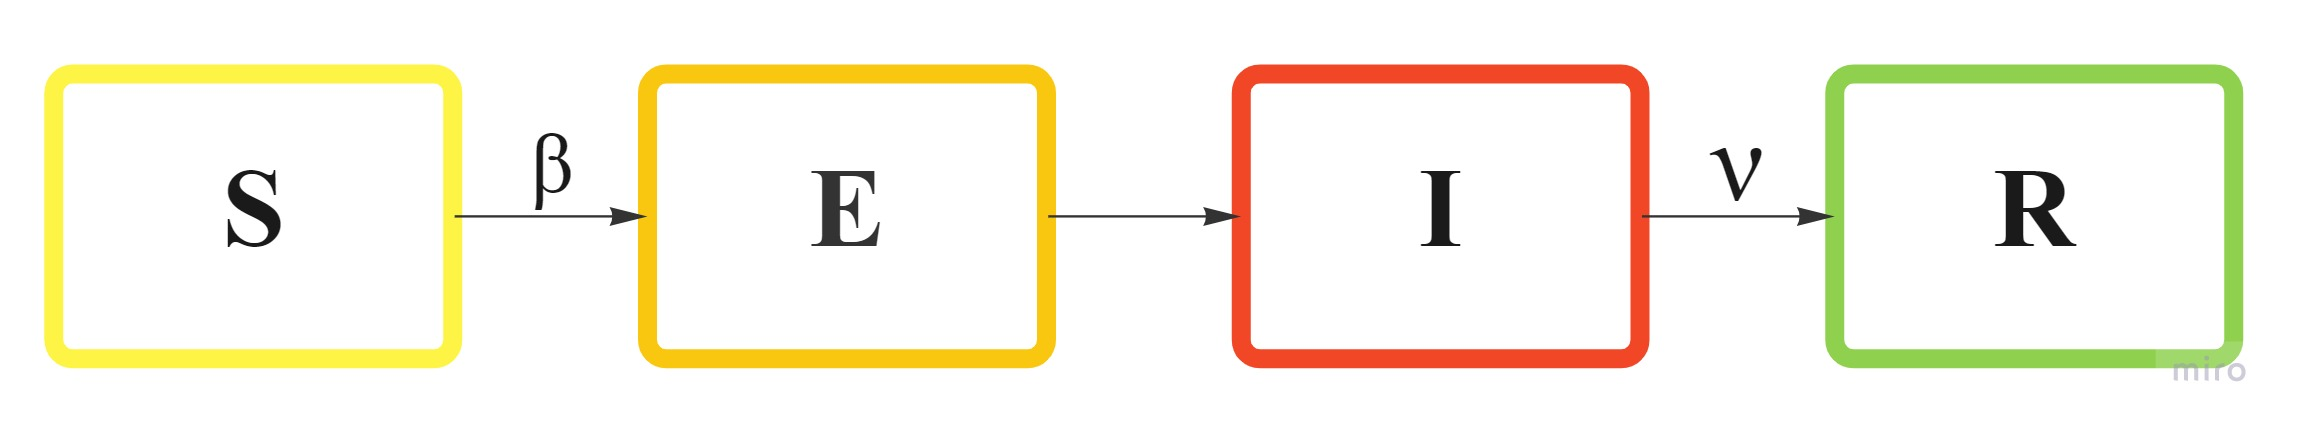
\includegraphics[width=0.9\textwidth]{Flowchart.jpg}
    \caption{Fluxograma do funcionamento geral do programa montado para a estimativa da Figura de Mérito. }
    \label{Fluxograma}
\end{figure}

Em ABM as unidades que interagem entre si, os agentes, apresentam diversas características como estado de saúde, idade, sexo, taxa de isolamento e entre outros que sejam necessários para a simulação, e são distribuídos de forma heterogênea em uma rede que representa uma população. A evolução da doença na rede depende de como cada agente interage com sua vizinhança e com outros agentes aleatórios. Em uma rede quadrada o contato entre os agentes podem ser representados das seguintes formas

\begin{itemize}
    \item Vizinhança de Von Neumman, os 4 vizinhos (norte, leste, sul, oeste).

    \item Vizinhança de Moore, todos os 8 vizinhos adjacentes ao agente.

    \item Contatos aleatórios.
\end{itemize}

Logo a probabilidade de contágio dependerá da vizinhança e do número de contatos aleatórios, e pode ser representada a partir da seguinte equação.

\begin{equation}\label{eqn:prob}
    \centering
    P = 1 - ( 1 - \beta)^n
\end{equation}
no qual n é quantidade de infecciosos que tiveram contato com o agente $\beta$ é a infecciosidade da doença que depende de $R_0$, parâmetro que representa quantos agentes são infectados a partir de um único caso. Um número aleatório $r_n$ é gerado, e caso $r_n$ < P, o agente é infectado.






\section{Arquitetura de GPUs}

Enquanto CPUs são orientadas para realizar operações mais complexas mas com baixa latência, GPUs são orientadas para maior \textit{throughput}, realizam operações mais simples, mas processam bastante tarefas ao mesmo tempo. Essas características tornam CPUs excelentes para tarefas em serial, enquanto GPUs são ótimas para tarefas paralelizaveis. Essa diferença ocorre devido a suas arquiteturas, CPUs tem poucos \textit{cores} que precisam de memória cache para diminuir a latência, enquanto GPUs não se preocupam tanto com latência, então possuem menos transístores para memória cache em benefício de mais transístores que realizarão processamento de tarefas, dependendo da família da GPU centenas e até milhares de \textit{cores} estão presentes.  



\begin{figure}[h!]
    \centering
    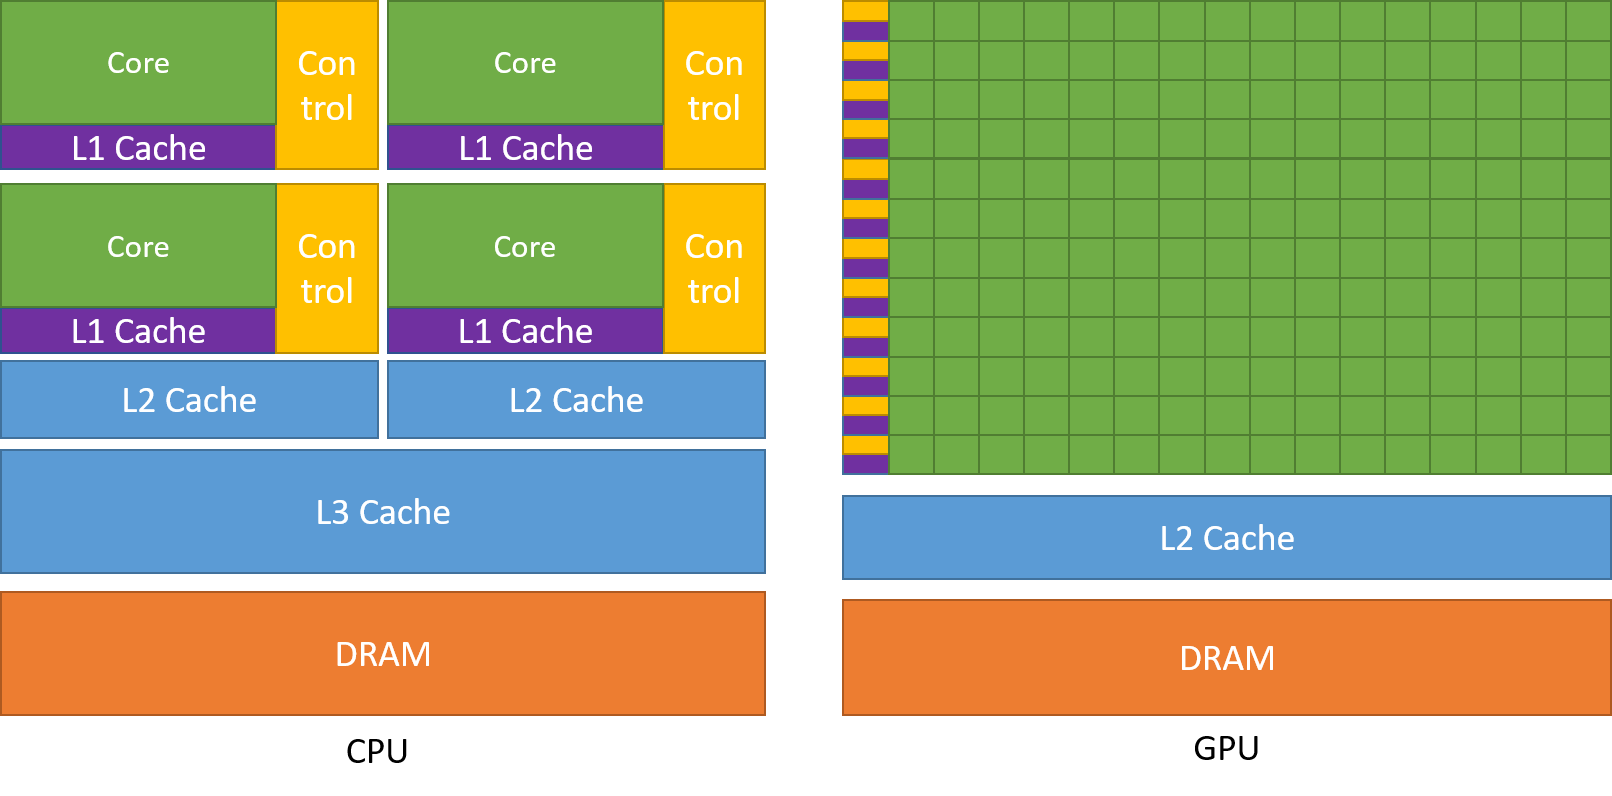
\includegraphics[width=0.9\textwidth]{gpu-devotes-more-transistors-to-data-processing.png}
    \caption{Arquitetura de uma CPU e de uma GPU. }
    \label{Fluxograma}
\end{figure}

GPUs contém SMs (\textit{streaming multiprocessors}), que contém CUDA \textit{cores} que realizarão as tarefas, cache L1, memória compartilhada entre os processadores dentro do SM e cache L2. Para obter maior \textit{throughput} os \textit{cores} nos SMs são SIMT (\textit{single instruction multiple thread}), para cada tarefa necessária um grupo de 32 \textit{cores} realizará a mesma tarefa, esses grupos são chamados de \textit{warps}, e o processamento da tarefas serão sempre realizados pela execução dos \textit{warps}.

\section{Modelo de progamação em CUDA}

CUDA é uma API (\textit{Application Programming Interface}) que permite a criação de programas em C/C++ em GPUs Nvidia que sejam compatíveis. Em CUDA o programador cria funções semelhantes as funções de C/C++, essas funções chamadas de kernels, realizam N tarefas para as N CUDA threads disponíveis na GPU utilizada. Um conjunto de threads é chamado de "blocks" e um conjunto de "blocks" forma um "grid", esses conjuntos podem ter até 3 dimensões. e podem ser identificados com variáveis nativas dadas por: \textbf{threadIDx, blockIdx,
blockDim} e \textbf{gridDim} manipulando essas variáveis o progamador consegue acessar e realizar tarefas para todas as threads.


Ao desenvolver programas utilizando a arquitetura CUDA, está-se envolvido em uma computação heterogênea, uma vez que o programa faz uso da interação entre a unidade central de processamento (CPU), também conhecida como \textit{host}, e a unidade de processamento gráfico (GPU), denominada como \textit{device}. No host o código é responsável para realizar as tarefas que precisam ser feitas em serial, alocações de memória, copiar os dados da memória da CPU para a GPU e então chamar os kernels para realizar as tarefas no device. Na GPU cada SM realizará as tarefas por bloco e após a finalização das execuções, o \textit{host} copia os resultados obtidos da memória da GPU para CPU. A Figura \ref{cuda} representa como funciona um programa feito em CUDA.

\begin{figure}[h!]
    \centering
    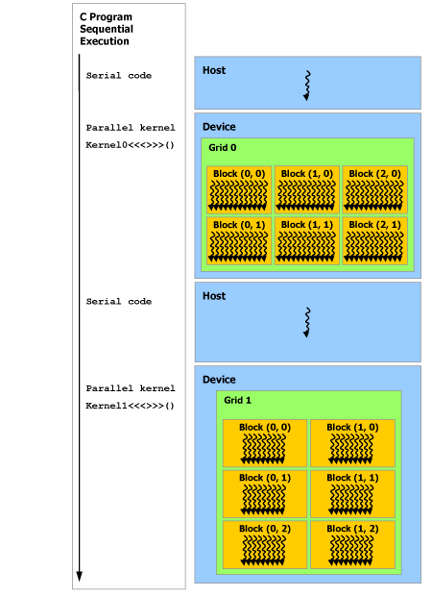
\includegraphics[width=10cm, height = 12cm]{heterogeneous-programming.png}
    \caption{Execução de um programa feito em CUDA. }
    \label{cuda}
\end{figure}










\chapter{Metodologia}
\label{Met}

\section{O Modelo}

A modelagem baseada em agentes utilizada será uma modificação do modelo compartimental SEIR, os indivíduos podem ter os seguintes estados de saúde, suscetíveis (X), expostos (E), pré-sintomáticos (P), assintomáticos (A), sintomático leve ($S_l$), sintomático moderado ($S_m$), sintomático severo ($S_s$), hospitalizado (H), internados na UTI (UTI), recuperados (R) e mortos (M). A Figura \ref{Fluxograma} abaixo demonstra como ocorre os possíveis movimentos dentre os estados de saúde.

\begin{figure}[h!]
    \centering
    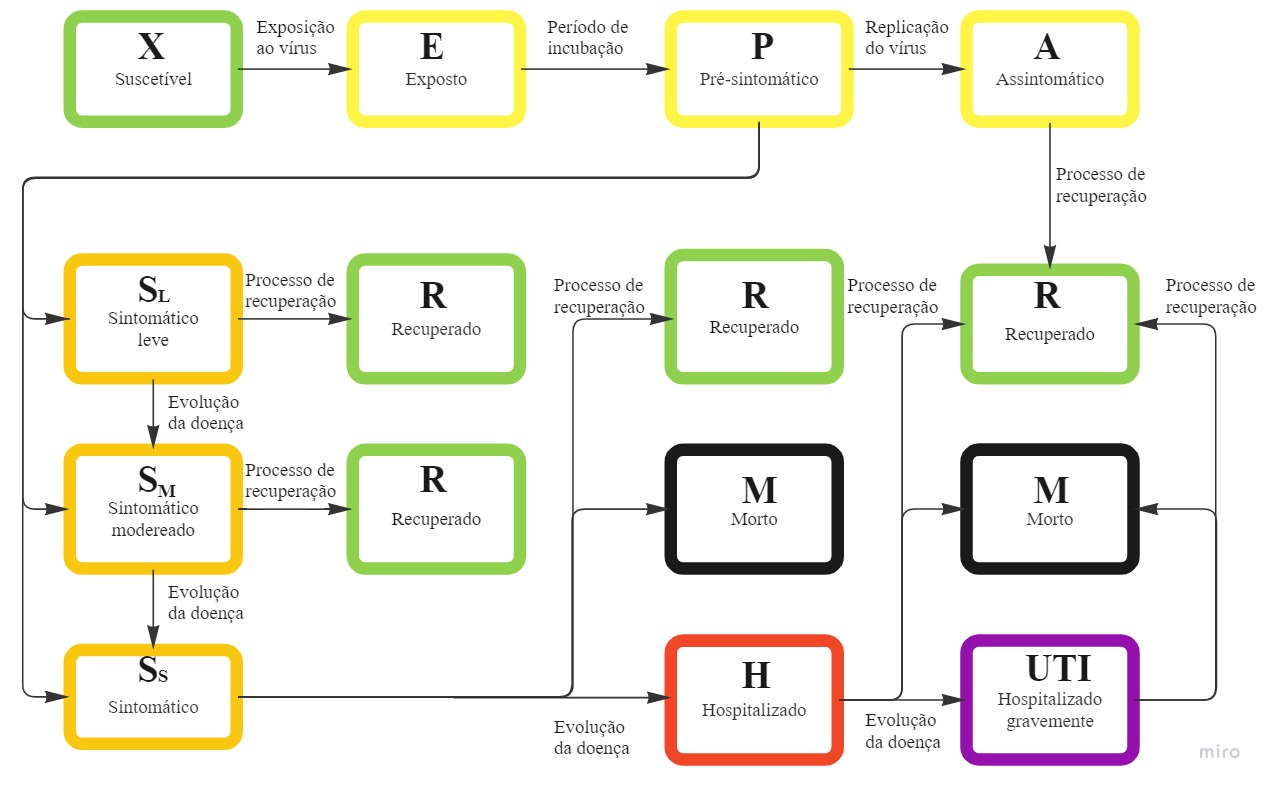
\includegraphics[width=0.9\textwidth]{covid fluxograma.jpg}
    \caption{Fluxograma do movimento entre estados de saúde. }
    \label{Fluxograma}
\end{figure}

O indivíduo suscetível (X) entra em contato com o vírus e torna-se exposto (E), após o período de incubação torna-se pré-sintomático (P), a replicação do virus ocorre e o indivíduo ou torna-se assintomático (A) e se recupera da doença, ou a doença evolui e o indivíduo se torna infeccioso, o indivíduo então pode ter sintomas leves ($S_l$), moderados ($S_m$) ou severos ($S_s$), caso não se recupere, será hospitalizado (H) e em casos mais graves internados em unidades de tratamento intensivo (UTI), na UTI o indivíduo ou se recupera, ou morre devido a doença.

No modelo cada indivíduo ocupa uma posição em uma matriz quadrada de lado L com poulação total $N = L X L$, tal que N é referente a cada cidade analisada. No inicio de cada simulação a população é iniciada com todos indivíduos com estado suscetível (X), exceto 5 indivíduos que estarão em estado pré-sintomático, os indivíduos infectados entrarão em contato com sua vizinhança, Von Neumann para as cidades de baixa densidade populacional ou Moore para cidades de alta densidade, além dos contatos com outros indivíduos aleatórios. A probabilidade de infecção dos indivídous suscetíveis é dada pela equação \ref{eqn:prob}, um número aleatório r é gerado e caso $r < P$, o indivíduo é infectado.

\section{Parâmetros}
Para cada cidade a ser utilizada no modelo, a calibração da infecciosidade $\beta$ é necessária para que seja padrão em todas as cidades que
$R_0$ = 3.5, a calibração é feita utilizando a média de indivíduos infectados a partir de um único caso para diferentes valores de $\beta$ até que se encontre o valor que mais se aproxima ao desejado.
É necessário também mudar os parâmetros que são específicos de cada cidade, são eles: tamanho da população, densidade populacional, contatos aleatórios, leitos de hospital e leitos de UTI. A Tabela \ref{tab:area} mostra as características de 4 cidades, São Paulo (SP), Manaus (AM), Brasilía (DF) e a favela da Rocinha (RJ).


\begin{table}[h]
 \centering
% distancia entre a linha e o texto
 \scalebox{0.95}{
 \begin{tabular}{ |l| |l| |l| |l| |l| |l|   }
\hline
 
    \multicolumn{1}{|p{2.350cm}|}{\textbf{Área} \centering } &
    \multicolumn{1}{|p{2.350cm}|}{\textbf{Densidade populacional} \centering } &
    \multicolumn{1}{|p{2.350cm}|}{\textbf{L} \centering } &
    \multicolumn{1}{|p{2.350cm}|}{\textbf{Leitos/Pop} \centering } &
    \multicolumn{1}{|p{2.350cm}|}{\textbf{Leitos de UTI/Pop} \centering } &
    \multicolumn{1}{|p{2.350cm}|}{\textbf{Contatos aleatórios} \centering } 
  \\  
\hline
    \multicolumn{1}{|p{2.350cm}|}{São Paulo \centering } &
    \multicolumn{1}{|p{2.350cm}|}{Alta \centering } &
    \multicolumn{1}{|p{2.350cm}|}{3355 \centering } &
    \multicolumn{1}{|p{2.350cm}|}{0,00247452 \centering } &
    \multicolumn{1}{|p{2.350cm}|}{0,00043782 \centering } &
    \multicolumn{1}{|p{2.350cm}|}{2-19 \centering } 
  \\
    \multicolumn{1}{|p{2.350cm}|}{Rocinha \centering } &
    \multicolumn{1}{|p{2.350cm}|}{Alta \centering } &
    \multicolumn{1}{|p{2.350cm}|}{264 \centering } &
    \multicolumn{1}{|p{2.350cm}|}{0,00055111 \centering } &
    \multicolumn{1}{|p{2.350cm}|}{0,00014592 \centering } &
    \multicolumn{1}{|p{2.350cm}|}{2-120 \centering }  
  \\
    \multicolumn{1}{|p{2.350cm}|}{Brasília \centering } &
    \multicolumn{1}{|p{2.350cm}|}{Baixa \centering } &
    \multicolumn{1}{|p{2.350cm}|}{1604 \centering } &
     \multicolumn{1}{|p{2.350cm}|}{0,00260879 \centering } &
    \multicolumn{1}{|p{2.350cm}|}{0,00040114 \centering } &
    \multicolumn{1}{|p{2.350cm}|}{2 \centering } 
    \\
    \multicolumn{1}{|p{2.350cm}|}{Manaus \centering } &
    \multicolumn{1}{|p{2.350cm}|}{Baixa \centering } &
    \multicolumn{1}{|p{2.350cm}|}{1343 \centering } &
    \multicolumn{1}{|p{2.350cm}|}{0,00187124 \centering } &
    \multicolumn{1}{|p{2.350cm}|}{0,00027858 \centering } &
    \multicolumn{1}{|p{2.350cm}|}{2 \centering } 
    \\
  \hline
 \end{tabular} 
}
\caption{Parâmetros de 4 diferentes áreas do Brasil. }\label{tab:area}
\end{table}



Já os parâmetros relacionados à doença são comuns a todas as áreas modeladas. A Tabela \ref{tab:dias} mostra a duração, em dias, o período de cada estado de saúde, a Tabela \ref{tab:prob} mostra a probabilidade de transição entre os estados de saúdes.

\begin{center}
\begin{longtable}{|l|l|l|}

\hline \multicolumn{1}{|c|}{\textbf{Parâmetro}} & \multicolumn{1}{c|}{\textbf{Descrição}} & \multicolumn{1}{c|}{\textbf{Duração (dias)}} \\
\hline 


$\tau_{l}$ & Período de latência & 0 - 27  \\
$\tau_{P}$ & Pré-sintomático & 0 - 14  \\
$\tau_{A}$ & Assintomático & 0 - 7  \\
$\tau_{S_l}$ &  Sintomático leve & 0 - 14  \\
$\tau_{S_m}$ & Sintomático moderado & 0 - 28  \\
$\tau_{S_s}$ & Sintomático severo & 0 - 4  \\
$\tau_{H}$ & Hospitalização & 7 - 45  \\
$\tau_{UTI}$ & UTI & 10 - 60  \\
\hline 

\caption{Parâmetros de duração de cada estado de saúde.} \label{tab:dias} \\
\end{longtable}

\end{center}


\begin{center}
\begin{longtable}{|l|l|l|}

\hline \multicolumn{1}{|c|}{\textbf{Parâmetro}} & \multicolumn{1}{c|}{\textbf{Transição entre estados}} & \multicolumn{1}{c|}{\textbf{Probabilidade}} \\
\hline 


$P_{(P\rightarrow A)}$ & Pré-sintomático para assintomático & 0.5  \\
$P_{(P\rightarrow S_l)}$ & Pré-sintomático para sintomático leve & 0.6  \\
$P_{(P\rightarrow S_m)}$ & Pré-sintomático para sintomático moderado & 0.2  \\
$P_{(P\rightarrow S_s)}$ & Pré-sintomático para sintomático severo & 0.2  \\
$P_{(S_l\rightarrow S_m)}$ & Sintomático leve para sintomático moderado& 0.1  \\
$P_{(P\rightarrow A)}$ & Sintomático severo para hospitalização & 0.75  \\
$P_{(P\rightarrow A)}$ & Internação em UTI & 0.25  \\

\hline 

\caption{Probabilidades de transição entre estados de saúde.} \label{tab:prob} \\
\end{longtable}
\end{center}

\section{Implementação em CUDA}

Para implemetação em CUDA mudanças nas redes serão necesárias para que o seu tamanho seja múltiplo de 32, e assim não causar divergência entre os warps. Como o modelo gera números aleatórios, em um programa em paralelo a função rand utilizada em C não é \textit{thread safe}, contudo CUDA oferece, através da biblioteca cuRAND, alguns pseudo geradores de números aleatórios. Com números aleatórios que sejam paralelizaveis e uma paralelização da rede de modo que as vizinhanças não sejam  desfeitas, uma paralelização do modelo baseado em agentes deve ser bem sucedida.




\bibliographystyle{unsrt}
\begin{thebibliography}{9}


\bibitem{textbook}
Merrill R. Introduction to Epidemiology. Jones & Bartlett Learning: London, United Kingdom, 2010.

\bibitem{textbook}
Keeling, M.J. and Rohani, P. (2008) Modeling infectious diseases in humans and animals. Princeton: Princeton University Press. 

\bibitem{texbook}
Sanders, J. and Kandrot, E. (2011) Cuda by example: An introduction to general-purpose GPU programming. Upper Saddle River: Addison-Wesley. 

\bibitem{textbook}
Cheng, J., Grossman, M. and McKercher, T. (2014) Professional CUDA® C programming. INpolis, IN: Wrox, a Wiley brand. 

\bibitem{url}
http://cnes2.datasus.gov.br/Mod\_Ind\_Tipo\_Leito.asp?VEstado=00		

\bibitem{url}
https://docs.nvidia.com/cuda/cuda-c-programming-guide/index.html

\bibitem{url}
https://docs.nvidia.com/cuda/curand/index.html



\end{thebibliography}

\end{document}
